\documentclass[professionalfonts, xcolor={usenames,svgnames,x11names,table}]{beamer}

\usetheme{SBUclass}
\usepackage{mypackages}
\usepackage{mycommands}


\title{\texorpdfstring{Language \& Technology}{Language and Technology}}
\subtitle{Lecture 4: Word-Based Models}
\author{Thomas Graf}
\institute{Stony Brook University\\\texttt{lin120@thomasgraf.net}}
\date{}


\begin{document}
\unnumbered{
\begin{frame}
	\titlepage
\end{frame}
}

\begin{frame}{Counting Words}
    \begin{itemize}
        \item Here's something nobody would ever call fun:\\
            \highlight{counting words in a text}.
        \item But word counts are easy for computers,\\
            and they are surprisingly useful:
            \begin{itemize}
                \item culturomics
                \item \emph{adsense} (online ad placement)
                \item word meaning
                \item authorship attribution
            \end{itemize}
        \item So let's see how that works.
    \end{itemize}
\end{frame}

\begin{frame}{Assembling a Corpus}
    \begin{description}
        \item[Corpus] a collection of texts
    \end{description}

    \begin{example}
        \begin{itemize}
            \item Collected works of Shakespeare
            \item All tweets between 2012 and 2016
            \item Google books
            \item Wall Street Journal (WSJ) corpus
            \item Brown corpus
        \end{itemize}
    \end{example}

    \begin{itemize}
        \item All applications of word counting models need \highlight{lots of text}.
        \item Corpora are collections of texts.
        \item Often they have been prepared for easy use with computers.
    \end{itemize}
\end{frame}

\begin{frame}[fragile]{Splitting a Corpus into Word Lists}
    \begin{itemize}
        \item Corpora usually consist of plain text files.\\
            \subpoint{think txt rather than doc or pdf}
        \item We can read in a text file and use a regular expression\\
            to break the string into a list of words.\\
            This is called \textbf{tokenization}.
    \end{itemize}
\begin{pythoncode}
    string = "The sun shone, having no alternative, on the nothing new."
    tokens = re.findall("\w+", str.lower(string))
    print(tokens)
    >>> ["the", "sun", "shone", "having", "no", "alternative", "on",
         "the", "nothing", "new"]
\end{pythoncode}

    \begin{itemize}
        \item But what do we do with that list?
    \end{itemize}
\end{frame}

\begin{frame}[fragile]{Counting Words}
    \begin{itemize}
        \item It is easy to count how often each word occurs.
    \end{itemize}
\begin{pythoncode}
    from collections import Counter
    counts = Counter(tokens)
    print(counts)
    >>> {"the": 2, "alternative": 1, "having": 1, "new": 1, "no": 1,
         "nothing": 1, "on": 1, "shone": 1, "sun": 1}
\end{pythoncode}
    \begin{itemize}
        \item More technically: for each word type we count its word tokens.
    \end{itemize}
    \begin{description}
        \item[word type] a word of a given language
        \item[word token] instance of the word in a text
    \end{description}
\end{frame}

\begin{frame}{Some Terminology: Unigrams and n-Grams}
    \begin{itemize}
        \item When we only count words in isolation,\\
              we are building a \highlight{unigram} model.
        \item Unigram models are a special case of \textbf{n-gram} models,\\
              which count sequences of words.
        \item We will learn more about n-gram models at a later point.
    \end{itemize}
\end{frame}

\begin{frame}{A Word Count Application: Culturomics}
    \begin{itemize}
        \item \textbf{Culturomics} is the quantitative study of cultural trends\\
            with the help of corpora.
        \item How does the frequency of specific words change over time?
        \item Let's try it ourselves with the \href{https://books.google.com/ngrams}{Google n-gram viewer}!
    \end{itemize}

    \begin{center}
        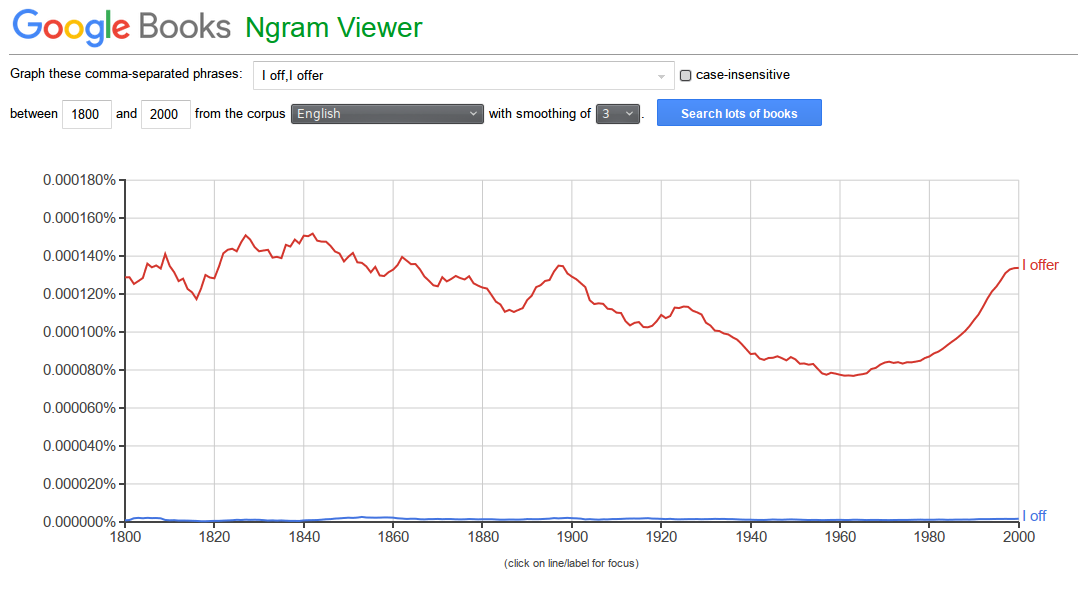
\includegraphics[width=1\linewidth]{./img/bigram_Ioff_Ioffer}
    \end{center}
\end{frame}

\begin{frame}{Careful: Don't Misinterpret the Data}
    \begin{itemize}
        \item The connection between language and culture is very indirect.
        \item Words have many meanings, we often don't know which meaning is tracked by frequencies.
    \end{itemize}
    \begin{exampleblock}{Example: Tracking Racism}
        \begin{itemize}
            \item \textbf{black} could also be color
            \item \textbf{chink} could be used for ``crack'', ``gap''
            \item \textbf{redskin} could be used for a fan of the sports team
        \end{itemize}
    \end{exampleblock}
    \begin{itemize}
        \item Additional problem: word meanings change over time
    \end{itemize}
\end{frame}

\begin{frame}{A Real-World Example of Language Change}
    \begin{center}
        
\includegraphics[width=1\linewidth]{./img/boner}
    \end{center}
\end{frame}

\begin{frame}{And There's More Where That Came From}
    \begin{center}
        \visible<1->{
\includegraphics[height=.4\linewidth]{./img/boner1}}
        \qquad
        \visible<2->{
\includegraphics[height=.4\linewidth]{./img/boner_2}}\\
        \visible<3>{
\includegraphics[width=.4\linewidth]{./img/boner_6}}
    \end{center}
\end{frame}


\begin{frame}{A Remark on Google Books}
	\begin{itemize}
		\item Google does tons of stuff with unigram and n-gram models.
		\item The more data they have, the better the models.
		\item When Google Books launched, people thought it was about
			\begin{itemize}
				\item extending Google's search business to books,
				\item creating a digital library,
				\item digital preservation.
			\end{itemize}
		\item Few realized it was all about getting\\
			  \highlight{more data for their models}!
	\end{itemize}
\end{frame}

\begin{frame}{Some Success Stories of Culturomics}
	Culturomics is still a young field, but there are interesting results:
		\begin{itemize}
			\item \textbf{Fukushima shift}\\
				Analysis of 5 million news paper articles reveals public shift on nuclear power after Fukushima accident.
			\item \textbf{Twitter forecast}\\
				Public sentiment can be reconstructed and traced via Twitter. 
			\item \textbf{Lexical point of no return}\\
				If a word does not disappear 30 to 50 years after its introduction, it is very unlikely to disappear at a later point.
		\end{itemize}
\end{frame}

\begin{frame}{Reasons to be Sceptical}
    \begin{itemize}
        \item As every new tool, culturomics is likely to be used incorrectly. 
        \item In particular, claims about public opinion are dubious.
        \item \textbf{Methodological issue:}\\
            How could we reliably falsify such claims?
        \item \textbf{Linguistic issue:} The occurrence of certain words in a sentence tells us very little about its meaning.
            %
            \begin{exe}
                \ex
                \begin{xlist}
                    \ex \textbf{Twitter post on sunny day:} What a lovely day!
                    \ex \textbf{Twitter post on rainy day:} What a lovely day!
                \end{xlist}
                \ex
                \begin{xlist}
                    \ex I'm asking you and Bill not to vote for Trump.
                    \ex I'm asking you and not Bill to vote for Trump.
                    \ex I'm not asking you and Bill to vote for Trump.
                \end{xlist}
            \end{exe}
    \end{itemize}
\end{frame}

\begin{frame}{Culturomics: The Jury is Still Out}
    \begin{itemize}
        \item Culturomics is a great tool as long as the questions are simple and restricted:
            %
            \begin{itemize}
                \item frequency of words and phrases over time
                \item trending topics
            \end{itemize}
            %
        \item But unigram/n-gram models are too limited for meaning.
        \item They make reliable claims about people's opinions\slash attitudes only if their shortcomings can be offset by enough data.
        \item No proof so far that large corpora solve the linguistic issues
    \end{itemize}

    \pause
    \begin{alertblock}{The Sceptic's Guide to Culturomics}
        \begin{itemize}
            \item Whether people talk about topic X is easy to study.
            \item What people think about topic X is much more difficult.
        \end{itemize}
    \end{alertblock}
\end{frame}

\begin{frame}{Learning More: Computational Sociology at Stony Brook}
    \begin{itemize}
        \item Jason Jones
        \item SOC 330 Media and Society
    \end{itemize}
    %
    \medskip
    \centering
    
\includegraphics[width=0.7\linewidth]{./img/jason}
\end{frame}

\begin{frame}{Application 2: Predicting the Success of Novels}
    \begin{columns}
        \column{.7\linewidth}
        \emph{Success with Style: Using Writing Style to Predict the Success of Novels}
        \begin{itemize}
            \item Study conducted here at Stony Brook by Vikas Ashok, Song Feng, and Yejin Choi
            \item \textbf{The Big Insight}\\
                Unigram models are surprisingly accurate at predicting the success of novels.
            \item \textbf{What it is \highlight{NOT} About}\\
                \begin{itemize}
                    \item computers writing successful novels
                    \item advice for becoming a successful author
                \end{itemize}
        \end{itemize}

        \column{.3\linewidth}
        \centering
        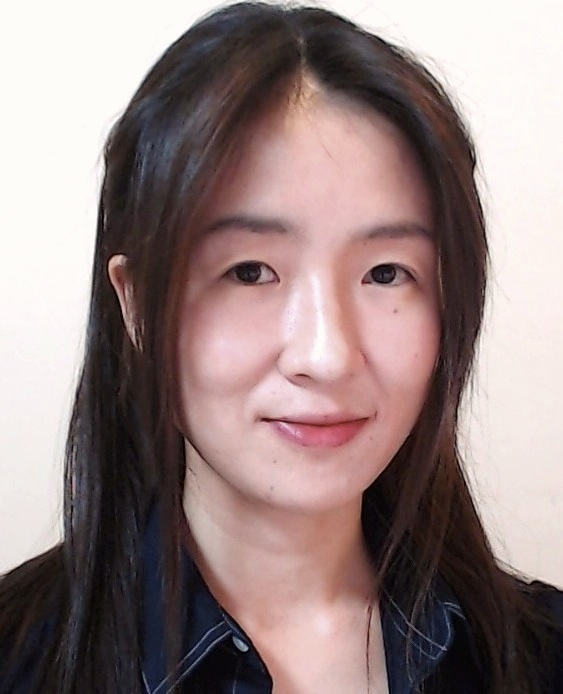
\includegraphics[width=1\linewidth]{./img/yejin_choi}
        \\
        \noindent
        \footnotesize\bfseries Yejin Choi
    \end{columns}
\end{frame}

\begin{frame}[fragile]{Methodology in Detail}
    % fixme: would be nice to have a flow chart of process here
    \begin{enumerate}
        \item<1-> collect books from Project Gutenberg
        \item<2-> annotate them as (un)successful\\
            \subpoint{mixture of financial turnout and critical evaluation}
        \item<3-> split annotated books into two groups\\
            \begin{itemize}
                \item \textbf{Training set}\\
                    used to train the model\slash learn frequencies\\
                \item \textbf{Test set}\\
                    used to test quality of the trained model
            \end{itemize}
        \item<4-> determine unigram frequencies in training set and\\
            establish statistical correlation to success of books
        \item<5-> get predictions of model for books in test set
        \item<6-> compare predictions to actual success\slash failure 
    \end{enumerate}
    %
    \begin{tikzpicture}[
        overlay,
        group/.style = {circle, thick, font=\bfseries,
                        draw=#1, fill=#1!25,
                        minimum size=6em}
        ]
        \node (books) [group={SteelBlue4}, visible on=<1>]
            at (26em,10em) {Books};

        % success
        \begin{scope}[yshift=-5em]
            \clip (22em,10em) rectangle (25.6em,18.5em);
            \node (success) [group={SeaGreen4}, visible on=<2>,
                             rotate=90, align=center]
                at (25.5em,15em) {Success\\ \\};
            
        \end{scope}

        % failure
        \begin{scope}[yshift=-5em]
            \clip (26.5em,10em) rectangle (30.1em,18.5em);
            \node (failure) [group={Red3}, visible on=<2>,
                             rotate=90, align=center]
                at (26.5em,15em) {\\ \\Failure};
        \end{scope}

        % training
        \begin{scope}
            % success
            \begin{scope}[yshift=-5em]
                \clip (22em,15.1em) rectangle (25.6em,18.5em);
                \node (success) [group={SeaGreen4}, visible on=<3->,
                                 rotate=90, align=center]
                    at (25.5em,15em) {Success\\ \\};
                
            \end{scope}

            % failure
            \begin{scope}[yshift=-5em]
                \clip (26.5em,15.1em) rectangle (30.1em,18.5em);
                \node (failure) [group={Red3}, visible on=<3->,
                                 rotate=90, align=center]
                    at (26.5em,15em) {\\ \\Failure};
            \end{scope}
        \end{scope}

        % test
        \begin{scope}
            % success
            \begin{scope}[yshift=-5em]
                \clip (22em,14.1em) rectangle (25.6em,10.5em);
                \node (success) [group={SeaGreen4}, visible on=<3->,
                                 rotate=90, align=center]
                    at (25.5em,14em) {Success\\ \\};
                
            \end{scope}

            % failure
            \begin{scope}[yshift=-5em]
                \clip (26.5em,14.1em) rectangle (30.1em,10.5em);
                \node (failure) [group={Red3}, visible on=<3->,
                                 rotate=90, align=center]
                    at (26.5em,14em) {\\ \\Failure};
            \end{scope}
        \end{scope}
    \end{tikzpicture}
\end{frame}

\begin{frame}{Findings}
    \begin{itemize}
        \item Unigram model made right prediction for
            $\approx$\highlight{75\%} of books
        \item More complicated models only marginally better ($\approx +2\%$)
        \item All models perform very badly on sci-fi and history. 
        \item All models perform much better on romance and adventure. 
        \item Successful books have a higher occurrence of \emph{and} and thought-oriented verbs like \emph{recognize} and \emph{remember}.
    \end{itemize}

    \pause
    \begin{block}{The Big Question}
        \begin{itemize}
            \item Those are interesting findings.
            \item But why do we find this? What does it mean?
        \end{itemize}
    \end{block}
\end{frame}

\begin{frame}{What it Doesn't Mean}
    \begin{columns}
        \column{.6\linewidth}
            \begin{itemize}
                \item Stand-up comedian \textbf{Dave Gorman}'s show \emph{Modern Life is Goodish} features what he calls found poems.
                \item \textbf{Idea:} collect outrageously stupid online comments into a poem
                \item In that spirit, here's some user comments from the \emph{Telegraph}.
            \end{itemize}

        \column{.4\linewidth}
        
\includegraphics[width=.8\linewidth]{img/dave_gorman}
    \end{columns}
\end{frame}

\begin{frame}{What it Doesn't Mean [cont.]}
    \begin{quote}
    Don't you think if there was a way to analyse what made a best-seller, authors would have figured it out long before a bunch of scientists with nothing better to do? There is not, and never will be, a way to write a best-selling novel. This comes from an author of fifteen years and a dozen novels.
    \end{quote}

    \visible<2>{
    \textbf{The Misunderstanding}\\
    \begin{itemize}
        \item This is not about writing successful books.
        \item The study is about predicting success of written books.
        \item The model is too abstract to be turned into writing advise.\\
            \subpoint{you cannot write with unigram frequencies}
    \end{itemize}
    }
\end{frame}

\begin{frame}{What it Doesn't Mean [cont.]}
    \begin{quote}
        This algorithm has an issue. 
        they are analyzing books which are SOLD!
        Not books which are on stock and should be sold.
        I means: How can a reader know how many ``adverbs'' or ``adjectives'' there are into a book, if the book is NOT yet bought by him??
        Thus once the book is ought, it's sold. And certainly the reader cannot bring the book back to store and claim the money back, because he doesn't like the book.
    \end{quote}

    \visible<2>{
    \textbf{The Misunderstanding}\\
    \begin{itemize}
        \item \emph{Nitpick 1}: you can return books
        \item \emph{Nitpick 2}: reviews and word-to-mouth drive sales
        \item \emph{Real issue}
            \begin{itemize}
                \item sold books are not part of the model at all
                \item this is a categorization task, categories happen to be success\slash failure
                \item the notion of success is not purely based on what sold
            \end{itemize}
    \end{itemize}
    }
\end{frame}

\begin{frame}{What it Doesn't Mean [cont.]}
    \begin{quote}
        These nitwits wanted their algorithm to discover whether a book (presumably in manuscript form) would be a ``commercial success'' --- so they used it to back-predict the ``commercial success'' of classics from Project Gutenberg? Good God!
        What made them think that the classics even *were* commercial successes [\ldots]
    \end{quote}

    \visible<2>{
    \textbf{The Misunderstanding}\\
        \begin{itemize}
            \item Again, this is only about predicting the right category.
            \item The authors call this category ``success'', and they define it in a reasonable manner (commercial and\slash or critical success).
            \item How well this lines up with what you consider success is irrelevant.
            \item ``Back-prediction'' is an essential part of model testing.
        \end{itemize}
    }
\end{frame}

\begin{frame}{What it Doesn't Mean [cont.]}
    \begin{quote}
        Perhaps the reason they found common threads in the successful novels is because they were well written....duh! Did we really need a computer algorithm to tell us that?
    \end{quote}

    \visible<2>{
    \textbf{The Misunderstanding}\\
        \begin{itemize}
            \item What does it mean to be well-written?
            \item How do you formalize it for a computer?
            \item The model has nothing to say about the quality of the writing style.
        \end{itemize}
    }
\end{frame}

\begin{frame}{What it Doesn't Mean [cont.]}
    \begin{quote}
        Such an algorithm would be impossible for a book written by one of the masters of English literature. It's only possible for junk books.
    \end{quote}

    \visible<2>{
    \textbf{The Misunderstanding}\\
        \begin{itemize}
            \item Many of the books on Project Gutenberg are literary classics.
            \item Why would this only work for junk books?\\
                The n-gram model can be used with any text.
        \end{itemize}
    }
\end{frame}

\begin{frame}{What it Doesn't Mean [cont.]}
    same guy as before, in a follow-up post:

    \begin{quote}
        I know what a computer algorithm is and it might be possible to ``write a book'' by this means if the book's ``formula'' was very simple indeed. But writing a great imaginative work of literature is not a step by step mechanical procedure and series of calculations by which a desired end is accomplished. That should be obvious to the meanest intelligence.
    \end{quote}

    \visible<2>{
    \textbf{The Misunderstanding}\\
        \begin{itemize}
            \item This is not about writing successful books.
            \item In particular, it is not about computers writing books.
        \end{itemize}
    }
\end{frame}

\begin{frame}{What it Doesn't Mean [cont.]}
    \begin{quote}
        The western world is now full of people who don't have jobs, but have employment. There is hardly a week goes by when some ``scientist'' after years of research states the bleeding obvious. 
        Meanwhile over in China they have the spanners and hammers out building things.
        They make lots of money, and we borrow it so that coco the clown can come up with pointless drivel like this.
    \end{quote}

    \visible<2>{
    \textbf{The Misunderstanding}\\
    \qquad o tempora, o mores
    }
\end{frame}

\begin{frame}{So What Does it Mean?}
    \begin{itemize}
        \item If we view the collection of successful books at a group level, there are statistical trends regarding unigram frequencies.
        \item These trends are pronounced enough that they are a good predictor for whether a specific book belongs to that group.
        \item But these trends do not necessarily explain why books are successful.
        \item \highlight{Correlation is not causation!}
    \end{itemize}
\end{frame}

\begin{frame}{Soap Box Slide: Public Science Writing}
    \begin{itemize}
        \item In defense of the commenters, the Telegraph article\\
            does a bad job summarizing the paper.
        \item This is a common theme with public science writing:\\
            they overhype and distort in their quest for clicks.
    \end{itemize}

    \begin{block}{Moral of the Story}
        \begin{itemize}
            \item Don't believe scientific news in mainstream media.
            \item Seek out specialized outlets:
                \begin{itemize}
                    \item science blogs
                    \item \href{https://www.quantamagazine.org/}{Quanta magazine}
                \end{itemize}
            \item Read the paper yourself (just the abstract and conclusion will already rectify the worst misconceptions).
            \item If the paper is behind a paywall
                \begin{itemize}
                    \item lobby congress to fund open access initiatives,
                    \item use \url{sci-hub.cc} (evil, evil piracy)
                \end{itemize}
        \end{itemize}
    \end{block}
\end{frame}

\begin{frame}{Soap Box Slide: The Telephone Game of Science Reporting}
    \centering
    \begin{tikzpicture}
        \node (scientist) at (0,0)
            [visible on=<2->]
            {
\includegraphics[width=.3\linewidth]{./img/scientist}};
        \node (paper) [right=8em of scientist]
            [visible on=<3->]
            {
\includegraphics[width=.3\linewidth]{./img/journal}};
        \node (university) [below=of paper]
            [visible on=<4->]
            {
\includegraphics[width=.3\linewidth]{./img/sbu}};
        \node (news) [left=8em of university]
            [visible on=<5->]
            {
\includegraphics[width=.3\linewidth]{./img/science_paper}};

        \foreach \Node/\Timer [remember=\Node as \previous (initially scientist)] in {%
            paper/3,
            university/4,
            news/5%
            }
            \draw[->,thick,visible on=<\Timer->] (\previous) to (\Node);
    \end{tikzpicture}
\end{frame}

\begin{frame}{Soap Box Slide: Group-Level and Individual-Level} 
    \begin{itemize}
        \item group-level predictions $\neq$ individual-level predictions
        %
    \end{itemize}
    %
    \begin{example}
        \begin{itemize}
            \item Math tests: men, as a group, outperform women, as a group.
            \item But the correlation between group and individual is weak.
            \item Gender is a bad predictor of an individual's math skills.
        \end{itemize}
    \end{example}
    %
    \begin{itemize}
        \item Many correlations only hold reliably at the group level\\
            (in particular those related to cognitive tasks).
        \item When they are strong enough to make for a useful predictor for individuals, that should grab your attention.
    \end{itemize}
\end{frame}
\end{document}
